\chapter{PX evaluation web application}
\label{ap:web_app}

A web application to manage \ac{PX} evaluations for \acp{PREG} was developed (See \autoref{fig:dashboard}). The application contains ten modules that allow Creating, viewing, updating and listing \ac{PX} evaluations for \acp{PREG} following the methodology presented in \autoref{ch:model}. The navigation diagram of the web application is presented in \autoref{fig:navigationDiagram}.

\begin{figure}[bth]
\myfloatalign
{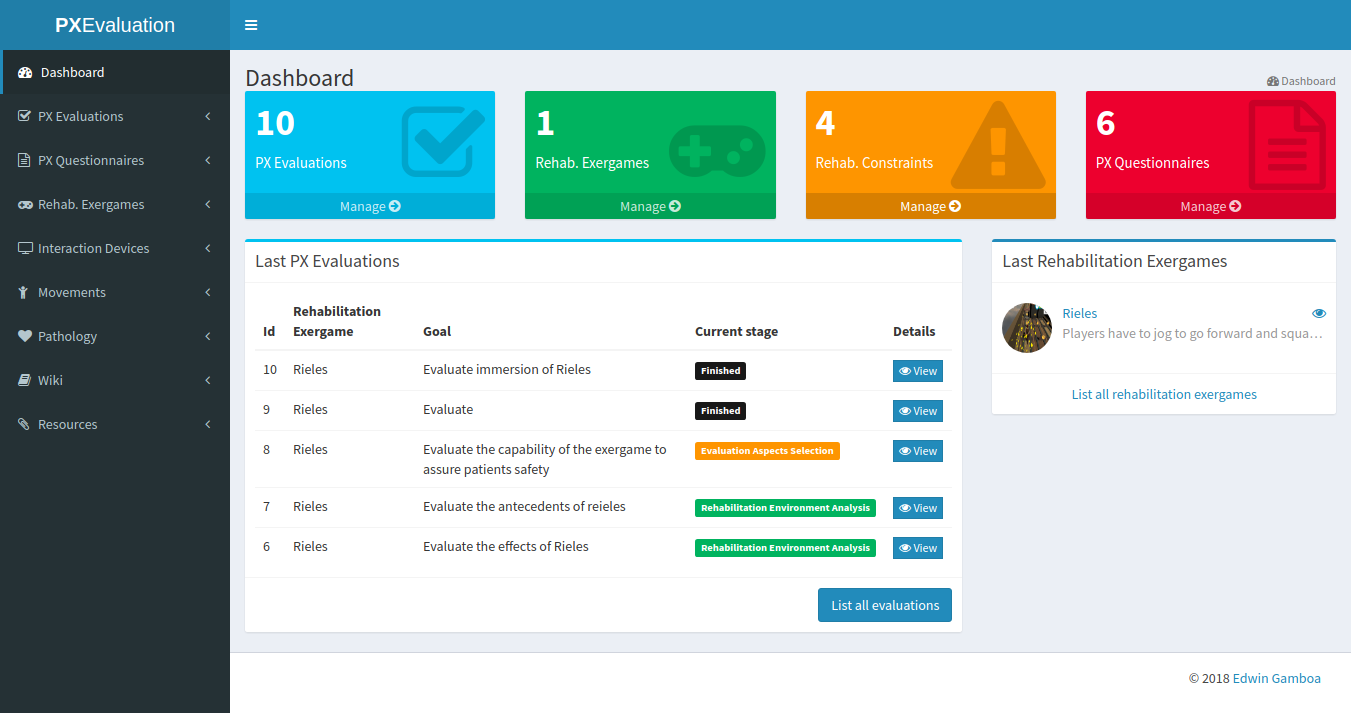
\includegraphics[width=\linewidth]{gfx/app/dashboard}} \quad
\caption{Dashboard of the \ac{PX} evaluation application}\label{fig:dashboard}
\end{figure}

\begin{figure}[bth]
\myfloatalign
{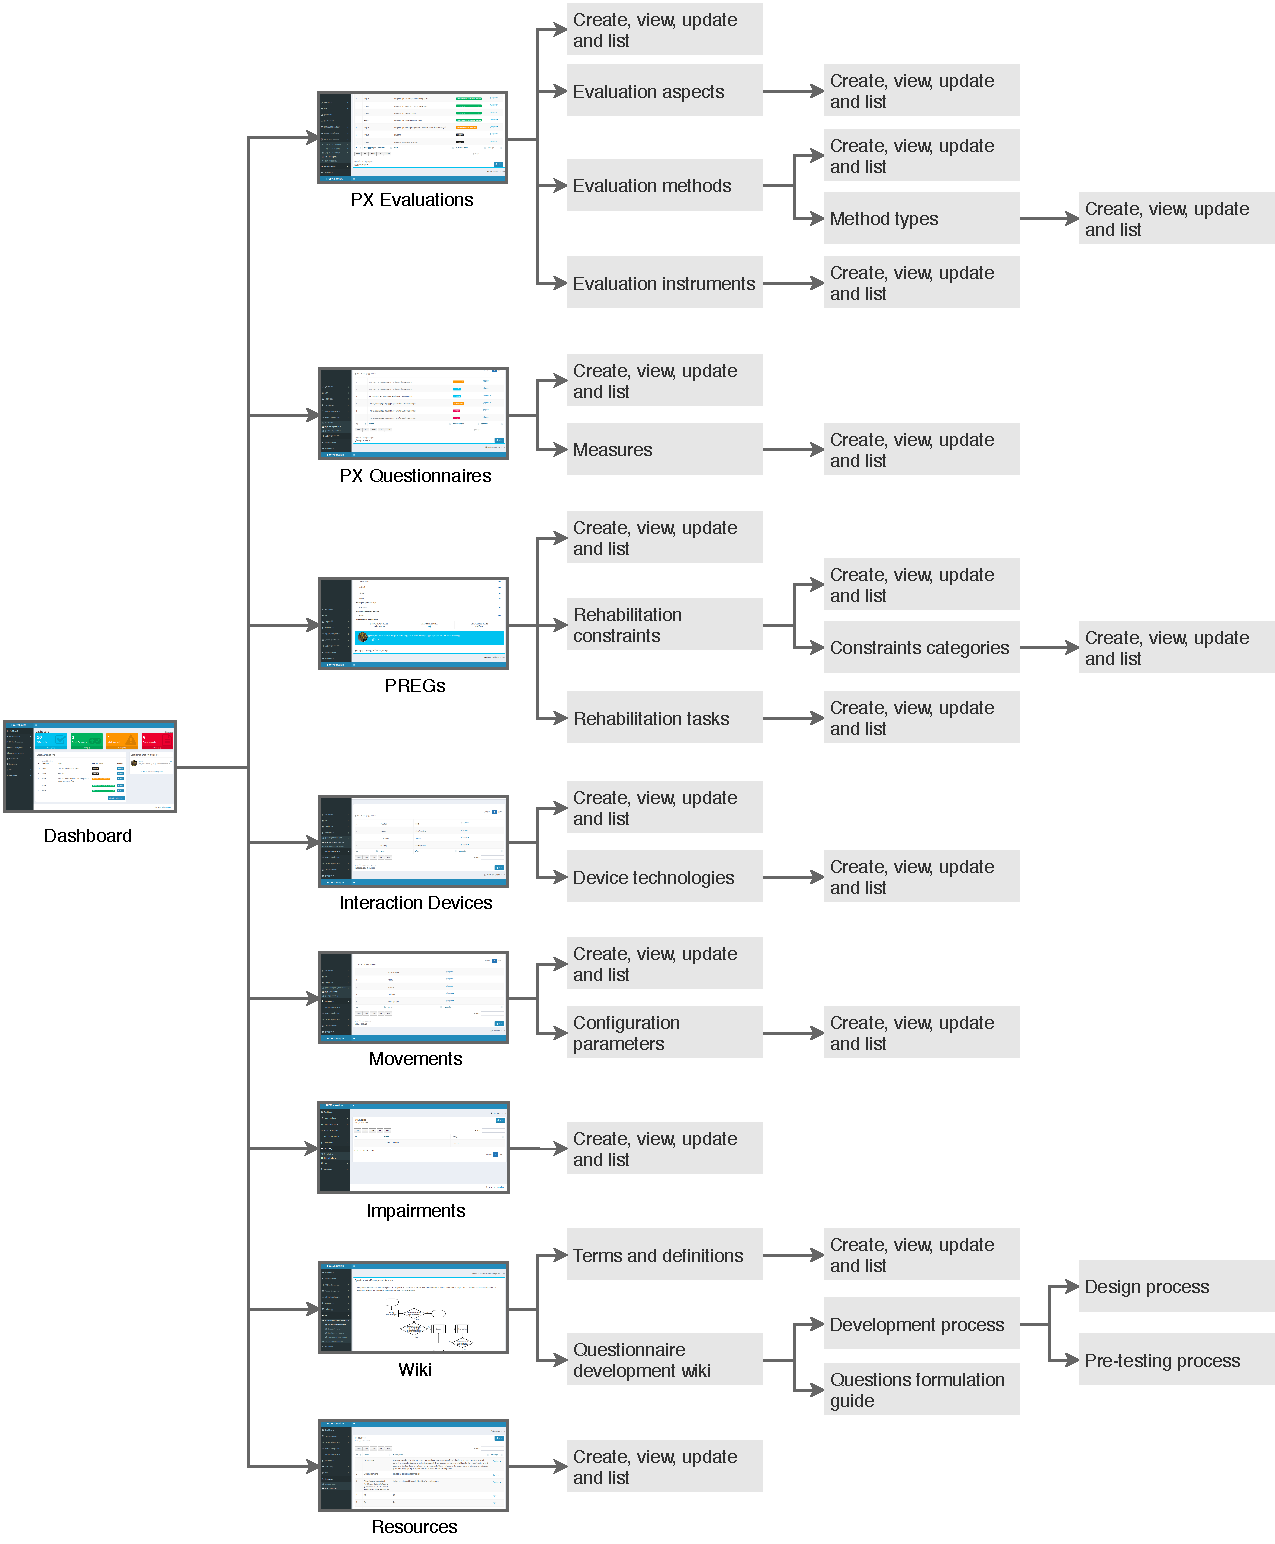
\includegraphics[width=\linewidth]{gfx/app/navigationDiagram}} \quad
\caption{Dashboard of the \ac{PX} evaluation application}\label{fig:navigationDiagram}
\end{figure}

The application was developed using the Django framework\footnote{Django Project: \url{www.djangoproject.com}}. The development process was conducted using agile practices including the use of a task-board, the creation of user stories, the use of semantic versioning and the management of issues. The development process was managed using the ZenHub\footnote{ZenHub: \url{https://www.zenhub.com/}} application and the code versioning was managed using git\footnote{Git: \url{https://git-scm.com/}} and GitHub\footnote{GitHub: \url{https://github.com/}}. The source code of the application is available online\footnote{Source code repository: \url{https://github.com/edwingamboa/rehab-exergames-px-app}}.


The web applications offers the following features:

\begin{enumerate}
    \item Creating (\autoref{fig:evaluationApp1}), viewing (\autoref{fig:evaluationApp2}), updating and listing \ac{PX} evaluations.
    \item Creating, viewing, updating and listing evaluation aspects.
    \item Creating, viewing, updating and listing evaluation methods.
    \item Creating, viewing, updating and listing types of evaluation methods.
    \item Creating, viewing, updating and listing evaluation instruments.
    \item Creating, viewing, updating and listing evaluation questionnaires, following the standard presented in \autoref{ch:questionnaire} (See \autoref{fig:standardApp}).
    \item Creating, viewing, updating and listing validation and reliability measures for questionnaires.
    \item Creating, viewing, updating and listing \acp{PREG} following the characterising approach presented in \autoref{sec:characterising} (See \autoref{fig:characterisingApp}).
    \item Creating, viewing, updating and listing rehabilitation constraints.
    \item Creating, viewing, updating and listing rehabilitation associated tasks (e.g, supervising and motivating).
    \item Creating, viewing, updating and listing interaction devices
    \item Creating, viewing, updating and listing device technologies.
    \item Creating, viewing, updating and listing rehabilitation movements.
    \item Creating, viewing, updating and listing configuration parameters.
    \item Creating, viewing, updating and listing impairments.
    \item Creating, viewing, updating and listing resources (e.g. documents such as evaluation reports, protocols, guides, among others).
    \item A wiki to read articles explaining the \ac{PX} evaluation methodology and the questionnaire standard.
    \item Creating, viewing, updating and listing terms and definitions to be used in the wiki.
\end{enumerate}

\begin{figure}[bth]
\myfloatalign
{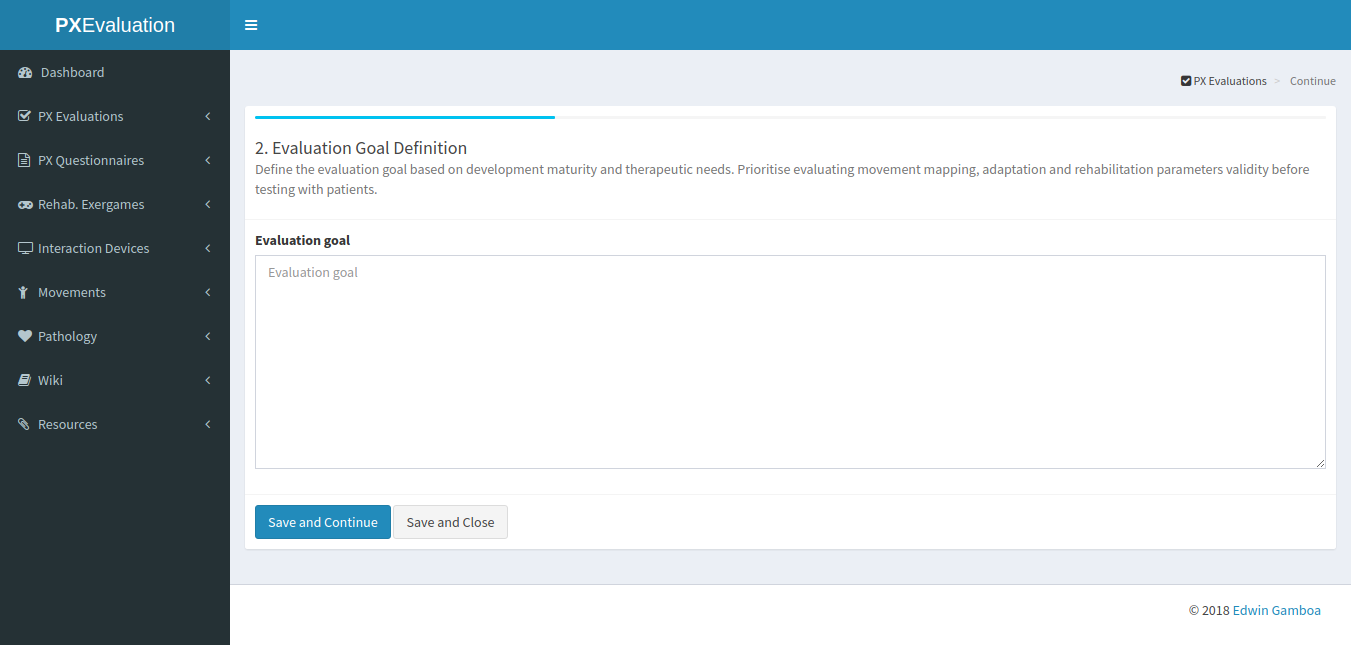
\includegraphics[width=.8\linewidth]{gfx/app/evaluationApp1}} \quad
\caption{Register view of an evaluation at the \ac{PX} evaluation application}\label{fig:evaluationApp1}
\end{figure}

\begin{figure}[bth]
\myfloatalign
{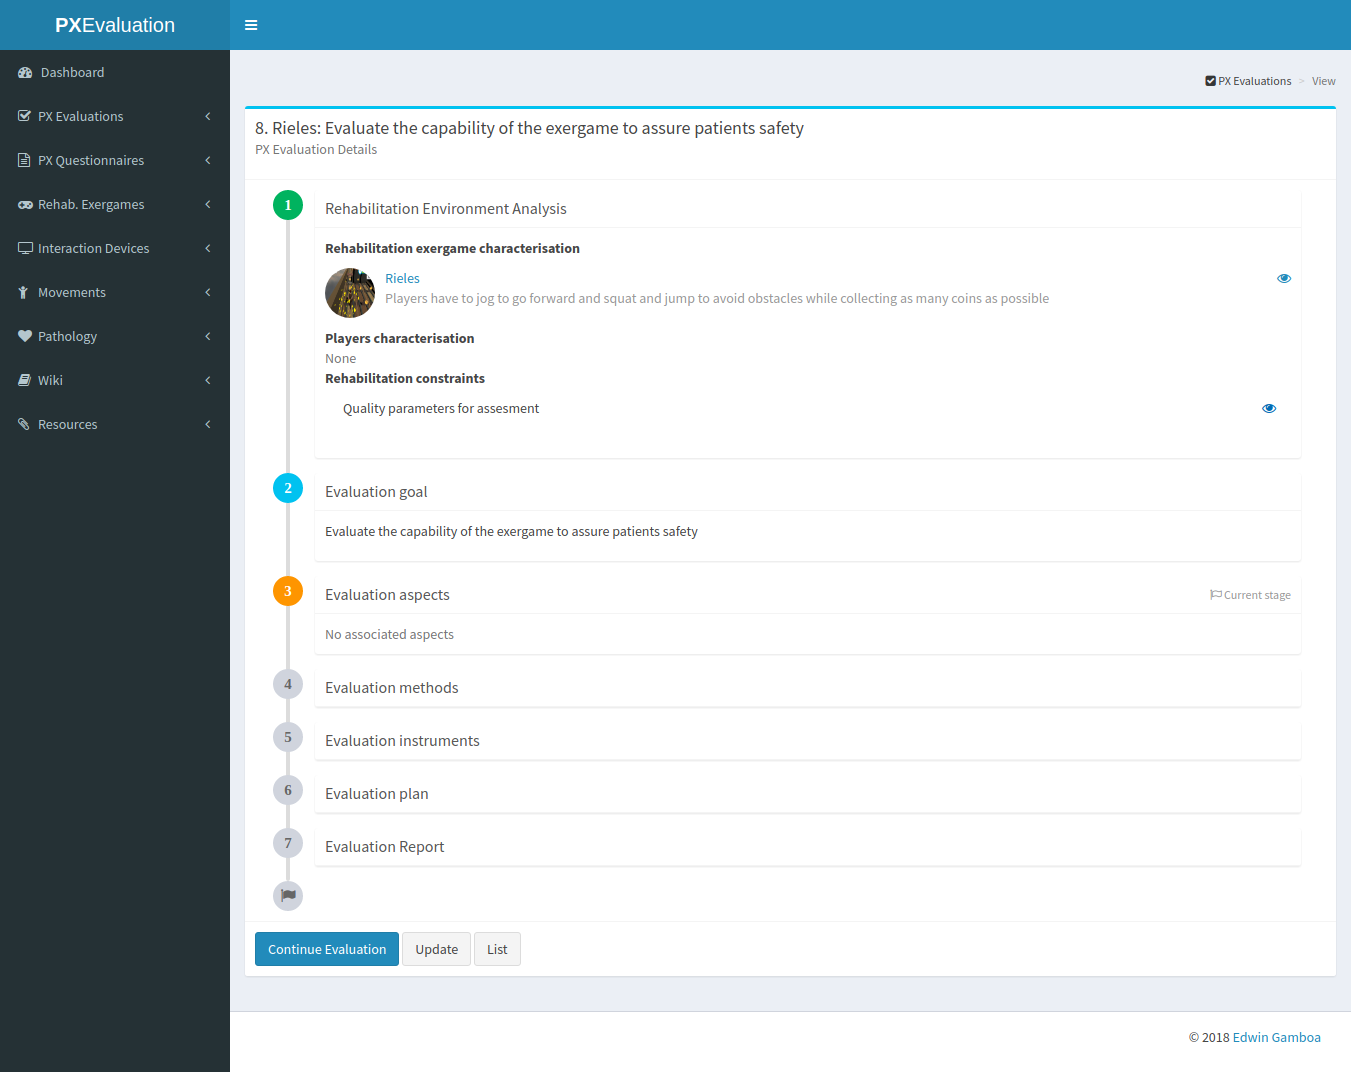
\includegraphics[width=.8\linewidth]{gfx/app/evaluationApp2}} \quad
\caption{Detail view of an evaluation at the \ac{PX} evaluation application}\label{fig:evaluationApp2}
\end{figure}


\begin{figure}[bth]
\myfloatalign
{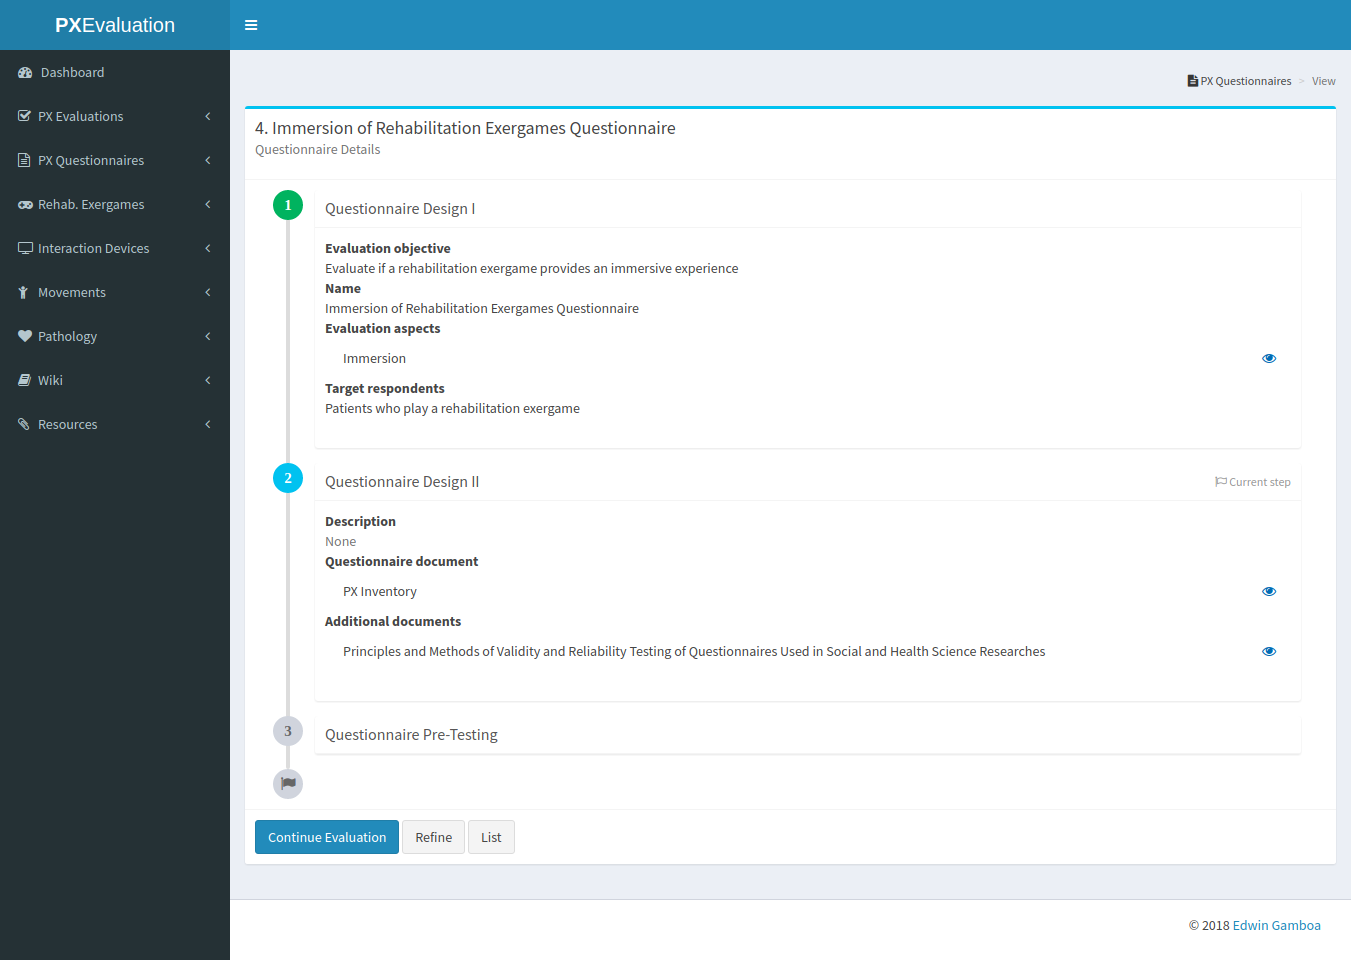
\includegraphics[width=.8\linewidth]{gfx/app/standardApp}} \quad
\caption{Detail view of a standard being developed at the \ac{PX} evaluation application}\label{fig:standardApp}
\end{figure}

\begin{figure}[bth]
\myfloatalign
{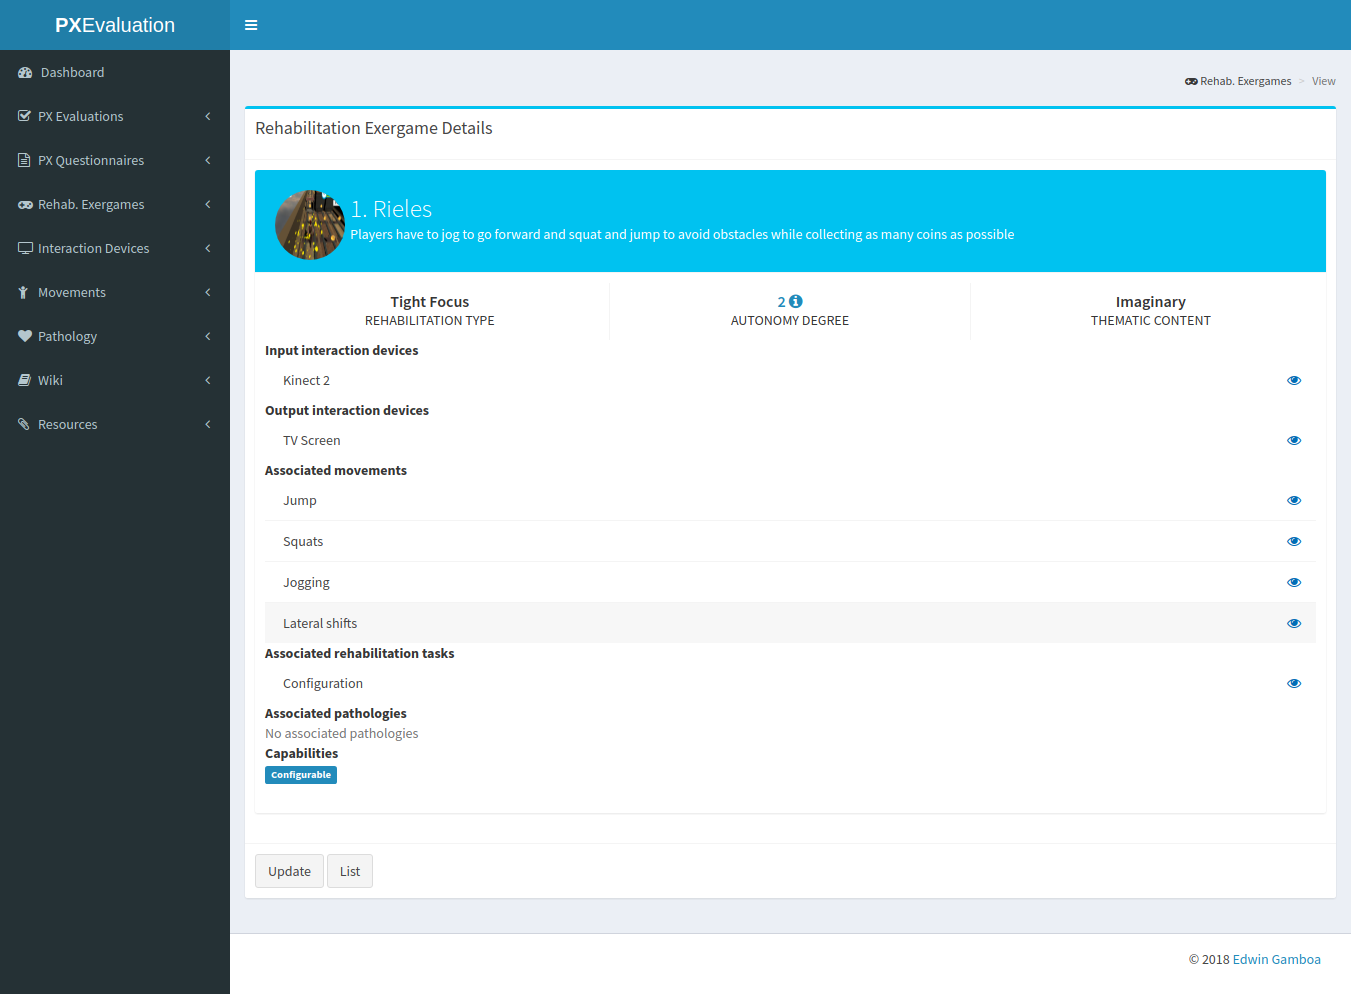
\includegraphics[width=.8\linewidth]{gfx/app/characterisingApp}} \quad
\caption{Detail view of a \ac{PREG} characterisation at the \ac{PX} evaluation application}\label{fig:characterisingApp}
\end{figure}
